\documentclass[11pt,a4paper]{article}
\usepackage[margin=2.3cm]{geometry}
\usepackage[T1]{fontenc}
\usepackage{lmodern}
\usepackage{amsmath,amssymb}
\usepackage{graphicx}
\usepackage{booktabs}
\usepackage{caption}
\usepackage{subcaption}
\usepackage[hidelinks]{hyperref}
\usepackage{cleveref}
\usepackage{xcolor}
\graphicspath{{../figures/}}
\newcommand{\todo}[1]{\textcolor{red}{[TODO: #1]}}
\newcommand{\Othree}{O$_3$}
\newcommand{\ugm}{$\mu$g/m$^3$}

\title{Denoising Low-Cost Ozone Sensors with Reference Subspaces and\\ Building Virtual Sensors with Graph Learning}
\author{Jose Arias\\ \small Topics on Optimization and Machine Learning (TOML), UPC -- BarcelonaTECH}
\date{\todo{date} \quad --- \quad DRAFT v0}

\begin{document}
\maketitle

\begin{abstract}
Low-cost sensors (LCSs) make dense air-quality monitoring possible, but even after in-situ calibration their measurements are noisier than those of reference instruments. This report covers two complementary techniques for improving data quality in a heterogeneous IoT monitoring network. First, we denoise calibrated ozone (\Othree) LCS data with a temporal-pattern-based approach inspired by \emph{eigenfaces}. Each day of sensor data is projected onto a low-dimensional subspace learned from reference-station days. With leave-one-day-out evaluation, projecting onto the RMSE-optimal subspace reduces the RMSE of an SVR-calibrated sensor from 12.46 to 11.65~\ugm{} ($-6.5\%$) and that of an MLR-calibrated sensor from 13.42 to 13.14~\ugm{} ($-2.2\%$). The Gavish--Donoho threshold selects a rank of $\kappa=7$ without using any co-located ground truth, and it loses less than 0.15~\ugm{} with respect to the optimal rank. Second, we learn the graph of a 12-node \Othree{} network in three ways (distance-based, graphical lasso and smoothness-based Laplacian learning) and use each graph to build virtual sensors from neighbouring nodes. The data-driven graphs need only about 4 neighbours per node to match the full-mesh baseline ($R^2\approx0.80$). Sparse distance-based graphs leave nodes isolated, which causes a large loss of accuracy.
\end{abstract}

%=====================================================================
\section{Introduction}
%=====================================================================
Air pollution is a major environmental health risk, and regulatory monitoring relies on reference stations. These stations are accurate but expensive, so they are deployed sparsely. Low-cost sensors (LCSs) can densify monitoring networks, but they suffer from cross-sensitivities, drift and noise, so they must be calibrated in situ against co-located reference instruments~\cite{spinelle2015,castell2017}. Calibration models such as multiple linear regression (MLR) or support vector regression (SVR) map the raw sensor signals to concentrations using only instantaneous measurements. They do not exploit the strong temporal structure of pollutants such as ozone, whose daily cycle is driven by solar radiation.

This report studies two ways of improving data quality in a heterogeneous network:
\begin{enumerate}
  \item \textbf{Denoising (TPB-D).} We treat each day of data as a vector, in the same way that eigenfaces treats each image as a vector~\cite{turk1991}. Calibrated LCS days are projected onto the subspace spanned by the dominant singular vectors of a database of reference-station days. We study how to choose the rank of this subspace, both with ground truth (minimum RMSE) and without it (the Gavish--Donoho hard threshold~\cite{gavish2014}).
  \item \textbf{Virtual sensors.} When a node fails or is never deployed, its signal can be reconstructed from its neighbours. The quality of the reconstruction depends on how the neighbourhood is defined. Following~\cite{ferrercid2021}, we compare a distance-based graph, a graphical-lasso (GLASSO) graph~\cite{friedman2008} and a Laplacian learned under a smoothness prior~\cite{dong2015,dong2016}. We then build MLR and SVR virtual sensors from each graph.
\end{enumerate}

The rest of the report is organised as follows. \Cref{sec:related} reviews related work, \cref{sec:methods} presents the methods and \cref{sec:data} the datasets. \Cref{sec:results} reports the results, and \cref{sec:conclusions} concludes.

%=====================================================================
\section{Related work}\label{sec:related}
%=====================================================================
\paragraph{Low-cost sensor calibration.} Field calibration of electrochemical \Othree{} and NO$_2$ sensors with linear and non-linear models was studied in~\cite{spinelle2015}. Large-scale evaluations of commercial platforms~\cite{castell2017} show that performance depends strongly on the calibration and on the deployment conditions. \todo{add the course references on in-situ calibration of O$_3$ LCS with MLR/SVR, e.g.\ the group's work on the CAPTOR / H2020 sensor networks.}

\paragraph{Subspace denoising.} Eigenfaces~\cite{turk1991} represents images as points in a low-dimensional linear subspace obtained by PCA/SVD. A new image is reconstructed by projecting it onto that subspace, which removes the components that are not explained by the training set. Choosing the rank is a classic problem. Gavish and Donoho~\cite{gavish2014} derived an optimal hard threshold for singular values under a Gaussian noise model. When the noise level is unknown, the threshold is a multiple $w(\beta)$ of the median singular value. \todo{cite the TPB-D/TPB-C paper from the course on which Figure 2 of the brief is based.}

\paragraph{Graph learning for sensor networks.} Graph signal processing (GSP) extends classical signal processing to signals defined on irregular structures~\cite{shuman2013,stankovic2019}. The graph can be fixed a priori from geometry (e.g.\ a thresholded Gaussian kernel of the distance~\cite{shuman2013}) or learned from the data. Statistical approaches estimate a sparse precision matrix of a Gaussian Markov random field with the graphical lasso~\cite{friedman2008}. GSP approaches learn a Laplacian under which the observed signals are smooth~\cite{dong2016,kalofolias2016}. Ferrer-Cid et al.~\cite{ferrercid2021} compared these families for air-pollution IoT platforms and used them to reconstruct signals at nodes that are missing.

%=====================================================================
\section{Methodology}\label{sec:methods}
%=====================================================================
\subsection{Calibration metrics}
Given reference values $y_t$ and estimates $\hat y_t$, $t=1,\dots,n$, we report
$\mathrm{RMSE}=\sqrt{\tfrac1n\sum_t(y_t-\hat y_t)^2}$ and
$R^2=1-\sum_t(y_t-\hat y_t)^2/\sum_t(y_t-\bar y)^2$.

\subsection{Temporal-pattern-based denoising (TPB-D)}
Let $\mathbf Y=[\mathbf y_1,\dots,\mathbf y_M]\in\mathbb R^{D\times M}$ contain $M$ reference days of $D=24$ hourly values each. Let $\boldsymbol\Psi=\frac1M\sum_i\mathbf y_i$ be the mean day, and let $\hat{\mathbf Y}=\mathbf Y-\boldsymbol\Psi\mathbf 1^\top=\mathbf U\boldsymbol\Sigma\mathbf V^\top$ be the SVD of the centred database. A calibrated LCS day $\mathbf x_i$ is denoised by projecting it onto the span of the first $\kappa$ left singular vectors:
\begin{equation}
  \tilde{\mathbf x}_i=\boldsymbol\Psi+\mathbf U_\kappa\mathbf U_\kappa^\top(\mathbf x_i-\boldsymbol\Psi).
  \label{eq:tpbd}
\end{equation}
For $\kappa=D$ the projection is the identity, so the denoised signal equals the calibrated signal. Small values of $\kappa$ force every day onto a few typical shapes.

\paragraph{Rank selection.} (i) \emph{RMSE-optimal}: $\kappa^\star=\arg\min_\kappa \mathrm{RMSE}(\mathbf Y,\tilde{\mathbf X}_\kappa)$, which requires co-located ground truth. (ii) \emph{Gavish et al.}~\cite{gavish2014}: $\tilde\sigma=w(\beta)\,\sigma_{med}$, with $w(\beta)\approx0.56\beta^3-0.95\beta^2+1.82\beta+1.43$ and $\beta=D/M$. The rank $\kappa$ is the number of singular values larger than $\tilde\sigma$.

\paragraph{Evaluation protocol.} If the day being denoised is also part of the reference database, its own reference profile lies inside the subspace, and the RMSE is optimistic. We therefore use \emph{leave-one-day-out}: day $i$ is denoised with a subspace (and mean $\boldsymbol\Psi$) computed from the other $M-1$ days.

\subsection{Graph construction}
For a network of $N$ nodes, each with $M$ samples, the graph is described by a weight matrix $\mathbf W$ or a Laplacian $\mathbf L=\mathbf D-\mathbf W$.
\paragraph{Distance-based.} We compute the haversine distances $d_{ij}$ (km) and set $w_{ij}=\exp(-d_{ij}^2/2\theta^2)$ if $d_{ij}<T$ and $w_{ij}=0$ otherwise. The threshold $T$ alone determines which links exist, while $\theta$ only sets their weights. Pruning on the weight instead ($w_{ij}\ge\epsilon$) is equivalent to the distance threshold $T=\theta\sqrt{2\ln(1/\epsilon)}$. \todo{confirm with the brief whether the kernel is $e^{-d/(2\theta)}$ or Gaussian; the conclusions do not change.}
\paragraph{GLASSO.} We assume the node signals are $\mathcal N(\mathbf 0,\boldsymbol\Sigma)$ and estimate a sparse precision matrix by solving
\begin{equation}
  \hat{\boldsymbol\Theta}=\arg\min_{\boldsymbol\Theta\succeq0}\ \mathrm{tr}(\mathbf S\boldsymbol\Theta)-\log\det\boldsymbol\Theta+\lambda\textstyle\sum_{j\neq k}|\Theta_{jk}|,
\end{equation}
where $\mathbf S$ is the sample covariance of the standardised data. Nodes $i$ and $j$ are linked if $|\hat\Theta_{ij}|>T$, with $T=10^{-4}$. We use \texttt{sklearn.covariance.GraphicalLasso}.
\paragraph{Laplacian learning~\cite{dong2015}.}
\begin{equation}
\begin{aligned}
  \min_{\mathbf L,\mathbf Y}\ & \|\mathbf X-\mathbf Y\|_F^2+\alpha\,\mathrm{tr}(\mathbf Y^\top\mathbf L\mathbf Y)+\beta\|\mathbf L\|_F^2\\
  \text{s.t. }& \mathrm{tr}(\mathbf L)=N,\quad L_{ij}=L_{ji}\le0\ (i\ne j),\quad \mathbf L\mathbf 1=\mathbf 0.
\end{aligned}
\end{equation}
The problem is not jointly convex, so we solve it by alternating minimisation. The $\mathbf L$-step is a convex QP in which $\mathrm{tr}(\mathbf Y^\top\mathbf L\mathbf Y)=\mathrm{tr}(\mathbf L\,\mathbf Y\mathbf Y^\top)$ is linear in $\mathbf L$; we solve it with CVXPY (Clarabel). The $\mathbf Y$-step has the closed form $\mathbf Y=(\mathbf I+\alpha\mathbf L)^{-1}\mathbf X$. We run three iterations, and the data are standardised with the quadratic term divided by $M$. In the first $\mathbf L$-step ($\mathbf Y=\mathbf X$) the minimiser depends only on the ratio $\beta/\alpha$.

\subsection{Virtual sensors}
For a target node $k$, the features are the signals of its graph neighbours $\{j:w_{kj}\ne0\}$. We train (i) MLR and (ii) an RBF-kernel SVR whose $C$ is chosen by three-fold time-series cross-validation. As baselines we use the \emph{full mesh} (all other 11 nodes) with MLR, Ridge and Lasso, where the regularisation strength is also chosen by time-series CV.

%=====================================================================
\section{Datasets}\label{sec:data}
%=====================================================================
\paragraph{Denoising dataset.} The data are hourly \Othree{} concentrations from 10 May to 5 October 2017 (2\,907 samples). They include the reference station (RefSt) and one LCS calibrated in situ with MLR and with SVR. No values are missing, but 669 of the 3\,576 hours in the period (18.7\%) have no row. After keeping only days with all 24 hours we obtain $M=104$ complete days out of 149 calendar days (22 days have no data and 23 are incomplete); see \cref{fig:days}.

\paragraph{Network dataset.} Hourly \Othree{} from 12 stations of the Catalan network (9 in the Barcelona metropolitan area and 3 in Osona, 40--78~km to the north), 1 June -- 6 October 2017, with $M=2\,170$ samples. The brief quotes $M=2\,258$, but the file contains 2\,170 rows. The timestamps in the file mix two formats, an Excel locale artefact: days $\le12$ are written month-first and days $>12$ day-first. We parsed them with this rule and verified that the result is monotonic. We split the data chronologically. The first 70\% (1 June -- 5 September, 1\,519 h) is used both to learn the graphs and to train the regressors, and the remaining 30\% (5 September -- 6 October, 651 h) is the test set.

%=====================================================================
\section{Results}\label{sec:results}
%=====================================================================
\subsection{Data exploration and in-situ calibration quality}
\Cref{fig:ts} shows the three signals. The diurnal cycle dominates: \Othree{} is low at night, rises after sunrise and peaks at 12--15~UTC. Both calibrated sensors track the reference closely, but MLR compresses the dynamic range. It overestimates low concentrations and saturates around 165~\ugm{}, whereas RefSt reaches 224~\ugm{} (\cref{fig:scatter}). SVR stays close to the 1:1 line over the whole range. \Cref{tab:calib} summarises the calibration quality.

\begin{table}[h]
\centering
\caption{In-situ calibration quality against RefSt.}\label{tab:calib}
\begin{tabular}{lcccc}
\toprule
 & \multicolumn{2}{c}{All hours ($n=2\,907$)} & \multicolumn{2}{c}{Complete days ($n=104\times24$)}\\
\cmidrule(lr){2-3}\cmidrule(lr){4-5}
Sensor & RMSE (\ugm) & $R^2$ & RMSE (\ugm) & $R^2$\\
\midrule
LCS -- MLR & 13.98 & 0.870 & 13.42 & 0.876\\
LCS -- SVR & 12.69 & 0.893 & 12.46 & 0.894\\
\bottomrule
\end{tabular}
\end{table}

\begin{figure}[t]\centering
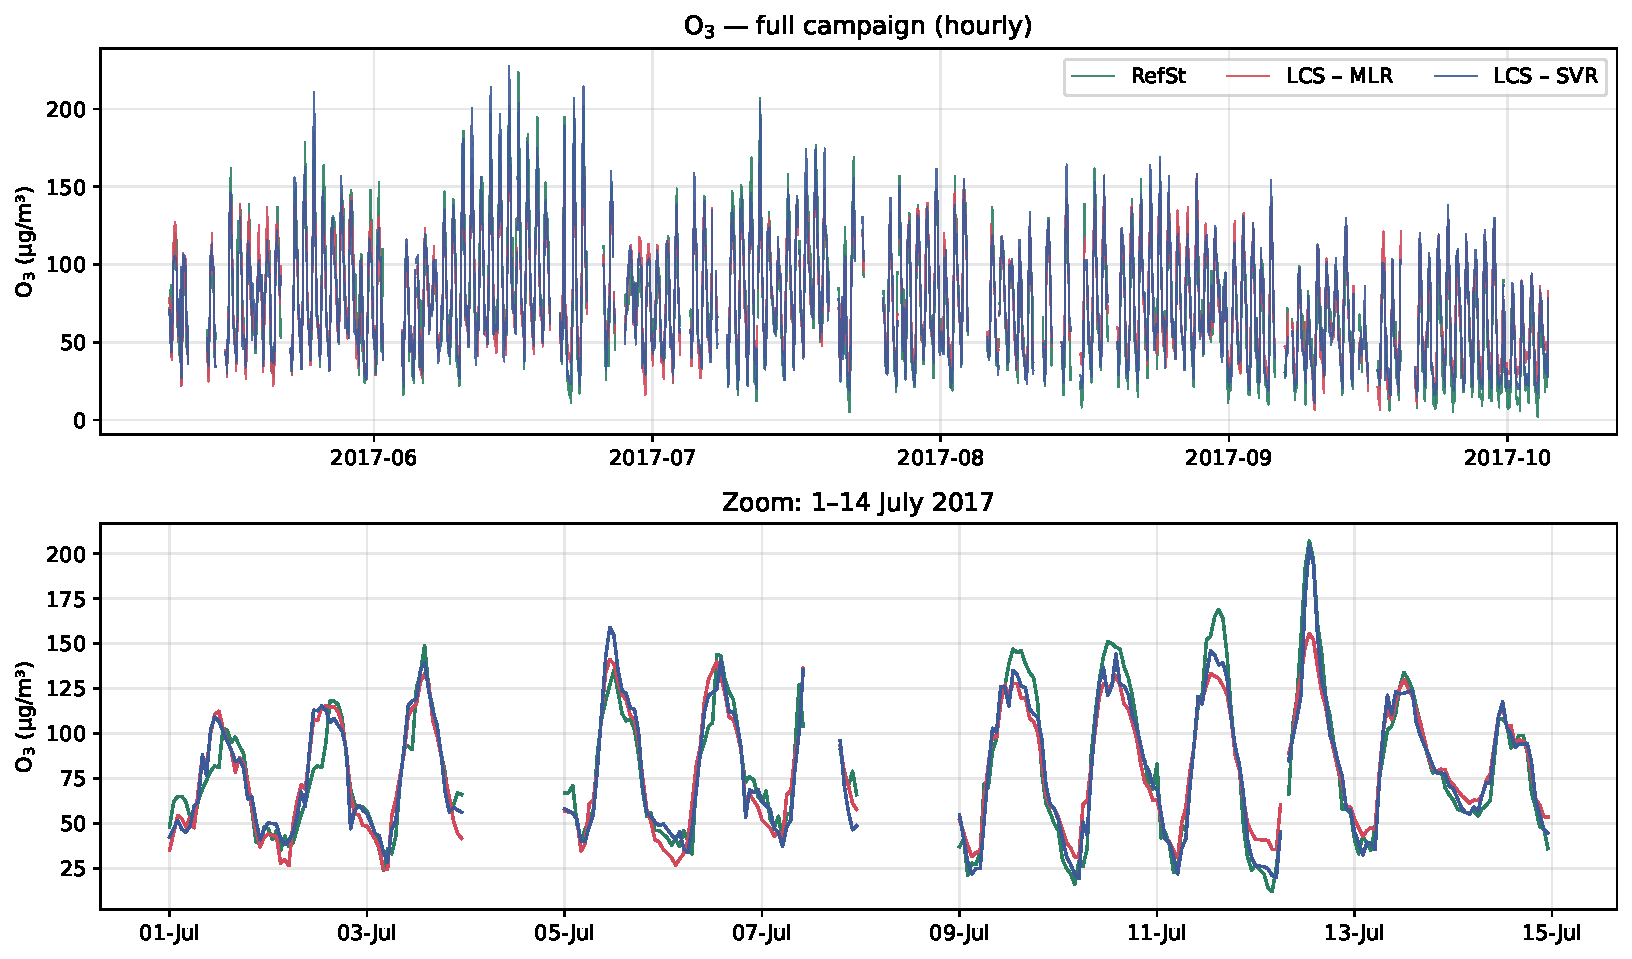
\includegraphics[width=\linewidth]{1_2_timeseries.pdf}
\caption{Reference and calibrated LCS \Othree{} over the full campaign (top) and a two-week zoom (bottom). Gaps are missing hours.}\label{fig:ts}
\end{figure}
\begin{figure}[t]\centering
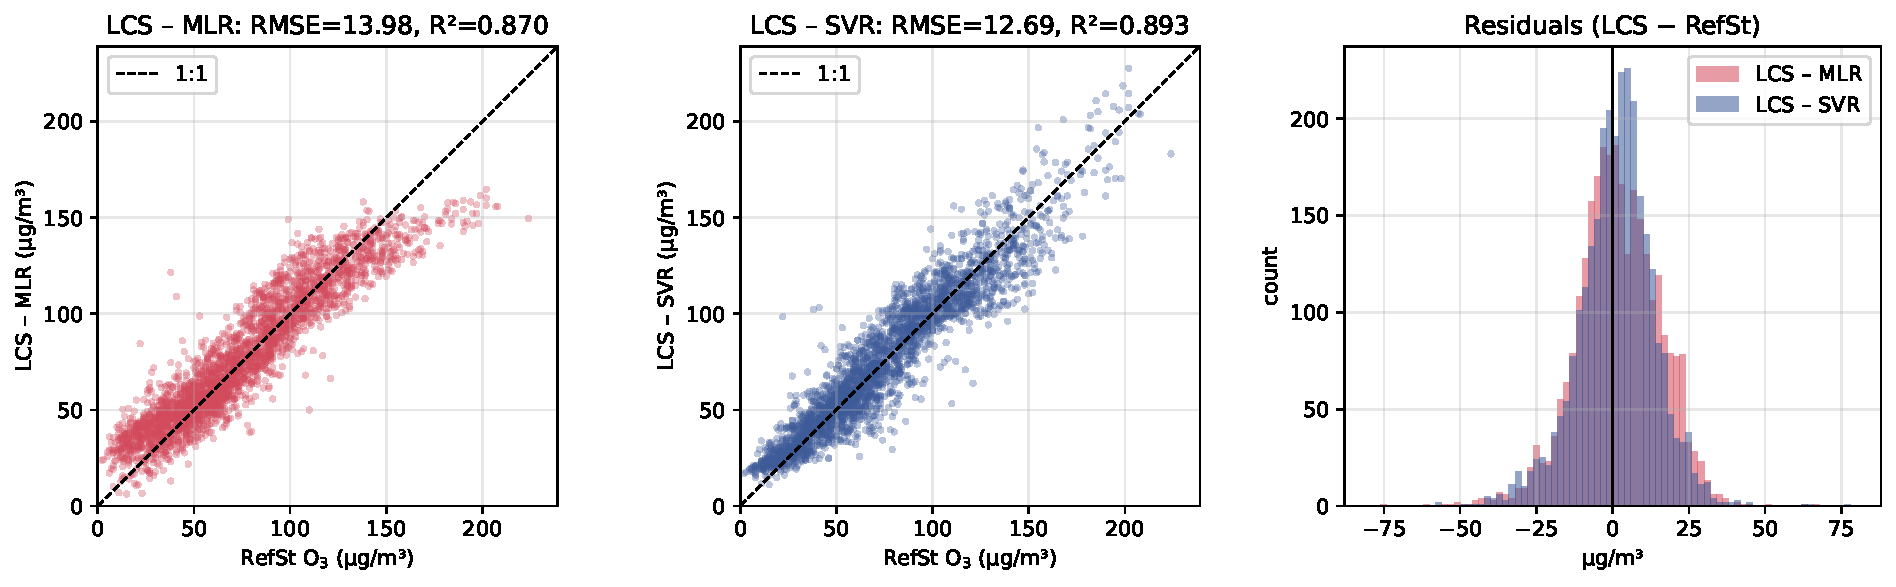
\includegraphics[width=\linewidth]{1_2_scatter_residuals.pdf}
\caption{Calibrated LCS vs RefSt and the residual distributions.}\label{fig:scatter}
\end{figure}
\begin{figure}[t]\centering
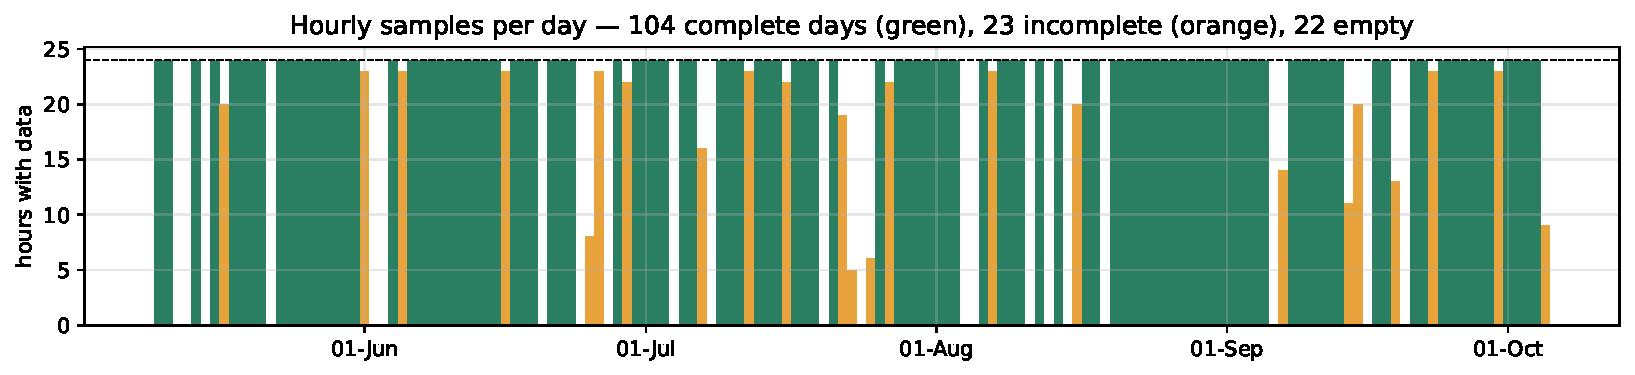
\includegraphics[width=\linewidth]{1_2_day_completeness.pdf}
\caption{Hourly samples per calendar day. Only the 104 complete days are used for denoising.}\label{fig:days}
\end{figure}

The error is not uniform during the day (\cref{fig:hour}). It is largest around the afternoon peak (16--18~\ugm{} at 12--15~UTC) and smallest at night. MLR also shows a jump at 6--9~UTC, when \Othree{} starts to rise. All daily profiles share the same shape (\cref{fig:overlay}), so a subspace built from a few typical days should describe them well.

\begin{figure}[t]\centering
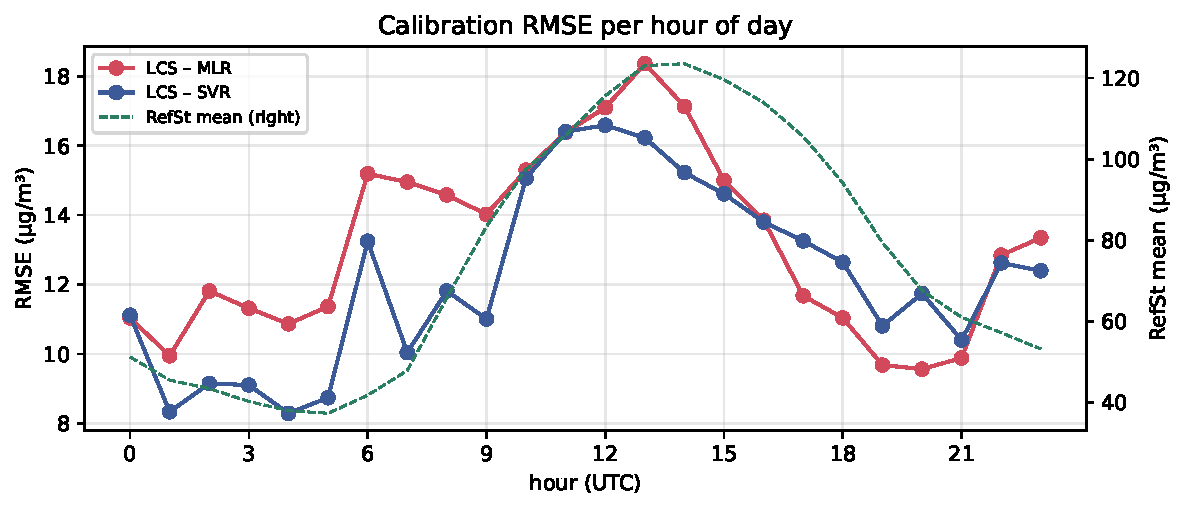
\includegraphics[width=0.75\linewidth]{1_2_rmse_by_hour.pdf}
\caption{Calibration RMSE for each hour of the day, with the mean RefSt profile (dashed, right axis).}\label{fig:hour}
\end{figure}
\begin{figure}[t]\centering
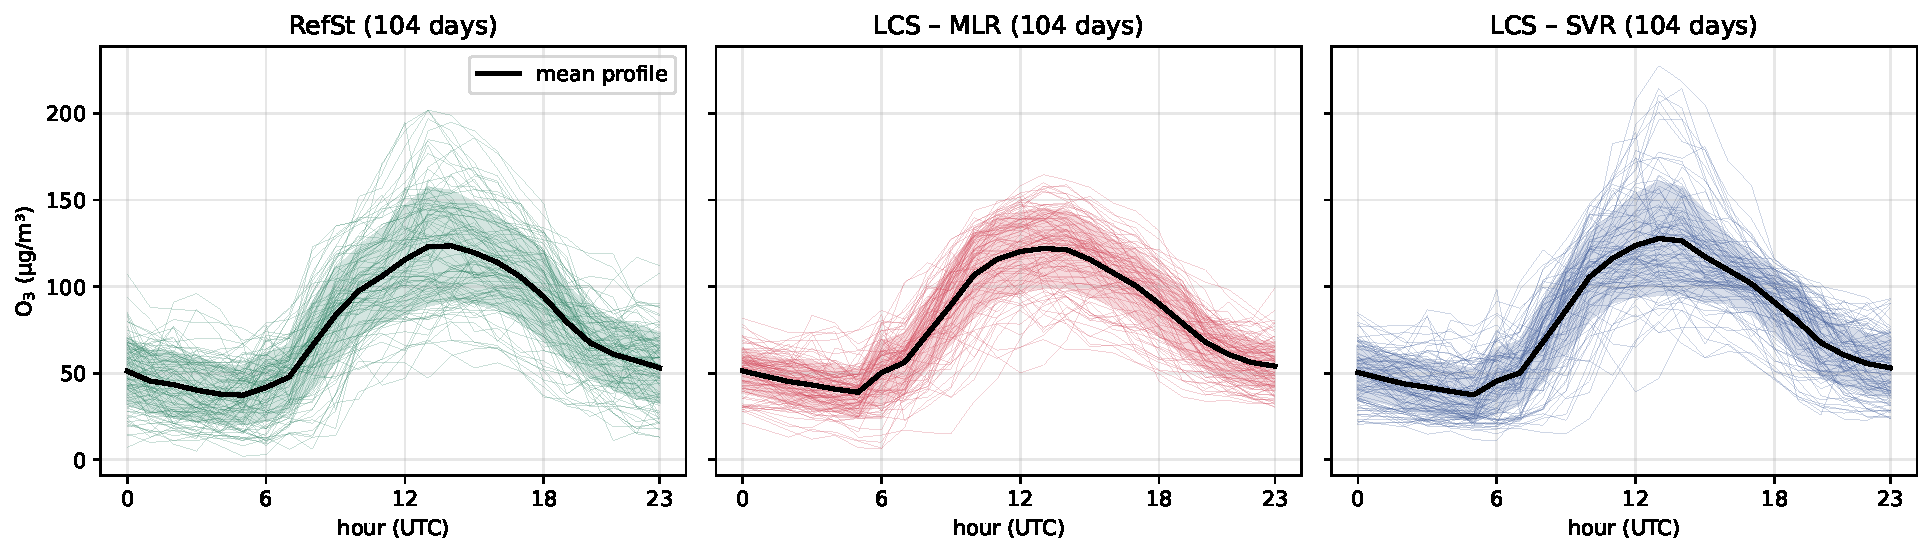
\includegraphics[width=\linewidth]{1_2_daily_overlay.pdf}
\caption{All 104 complete days overlaid, with the mean profile and a $\pm1\sigma$ band.}\label{fig:overlay}
\end{figure}
\begin{figure}[t]\centering
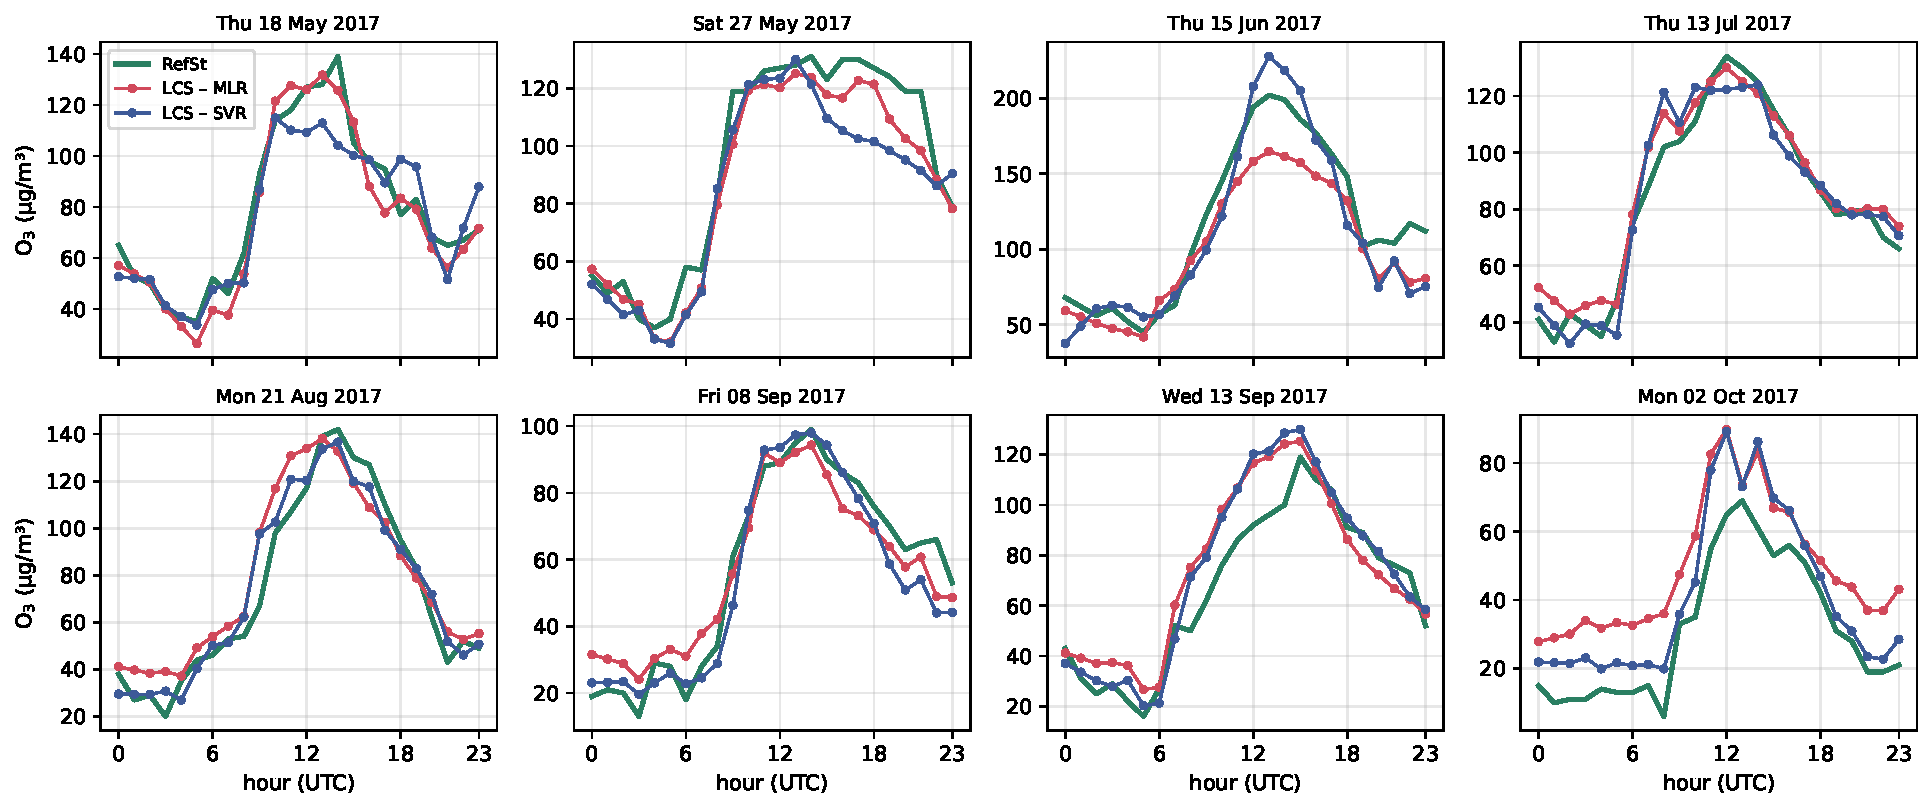
\includegraphics[width=\linewidth]{1_2_daily_examples.pdf}
\caption{Example days with low to high \Othree{} levels: RefSt vs the MLR and SVR calibrated LCS.}\label{fig:dayex}
\end{figure}

\subsection{Denoising}
\paragraph{Reference subspace.} The centred reference database is strongly low-rank (\cref{fig:svd}). The first singular vector explains 62\% of the variance and the first three explain 84\%. The first eigen-day $u_1$ (the sign is arbitrary) modulates the overall daytime level around the 13~UTC peak. $u_2$ contrasts night with afternoon and so controls the amplitude of the diurnal cycle. $u_3$ contrasts morning with evening and shifts the timing of the peak.

\begin{figure}[t]\centering
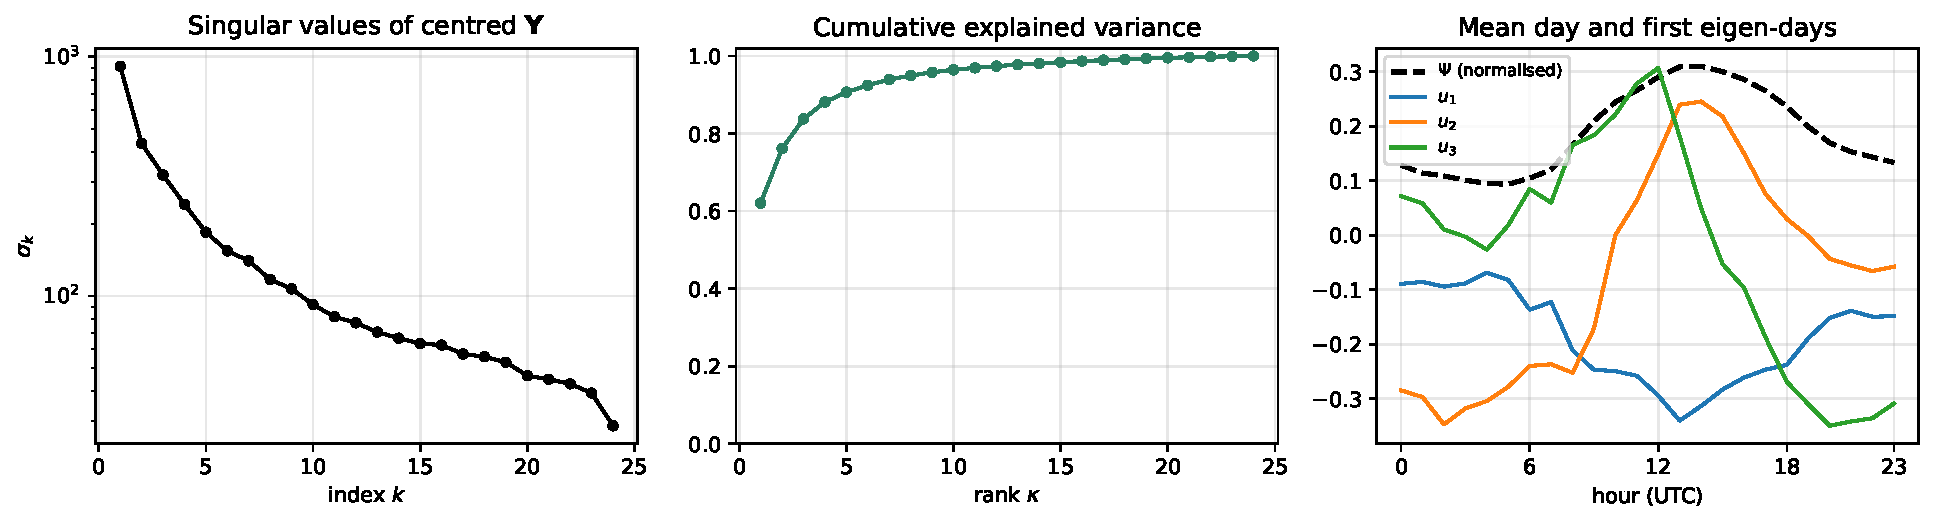
\includegraphics[width=\linewidth]{1_3_svd.pdf}
\caption{SVD of the centred reference daily database: singular values, cumulative explained variance, and the mean day with the first three eigen-days.}\label{fig:svd}
\end{figure}

\paragraph{Rank selection.} \Cref{fig:rmserank} shows the RMSE of the denoised sensors as a function of $\kappa$. The curve has the expected U shape. For small $\kappa$ the reconstruction is biased, because there are too few shapes to represent a particular day. For large $\kappa$ the projection lets the sensor noise back in, and at $\kappa=24$ the RMSE equals that of the calibrated sensor. The leave-one-day-out minimum is at $\kappa^\star=8$ for SVR and $\kappa^\star=10$ for MLR. The in-sample curve is consistently lower and illustrates how optimistic it is to include the day under test in the database.

\begin{figure}[t]\centering
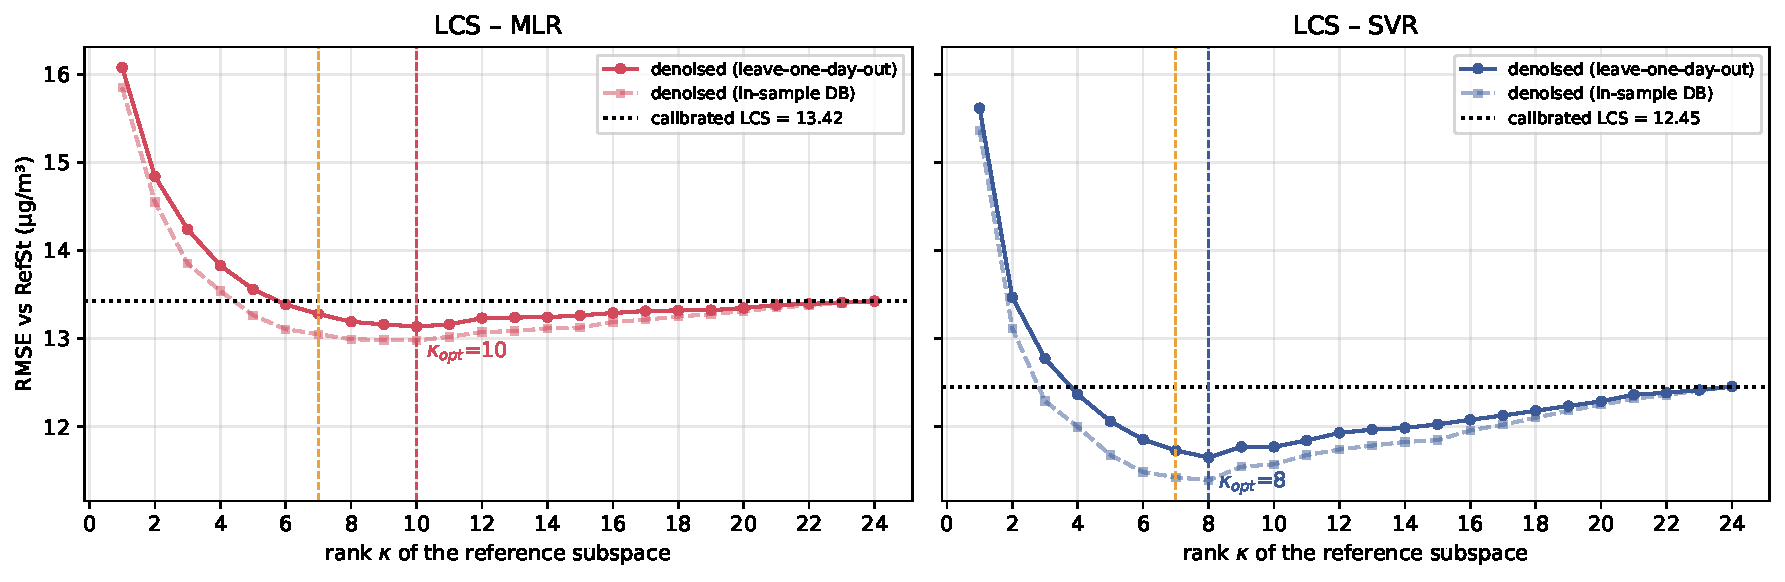
\includegraphics[width=\linewidth]{1_3_rmse_vs_rank.pdf}
\caption{RMSE of the denoised LCS vs the rank of the reference subspace. The dotted line is the calibrated sensor (no denoising). The vertical lines mark the RMSE-optimal rank (blue/red) and the Gavish et al.\ rank (orange).}\label{fig:rmserank}
\end{figure}

\paragraph{Gavish et al.\ threshold.} With $D=24$ and $M=104$, $\beta=0.231$ and $w(\beta)=1.806$. The median singular value is $\sigma_{med}=73.99$, which gives the threshold $\tilde\sigma=133.6$ and $\kappa_{G}=7$ (\cref{fig:gavish}). The same value is obtained in all 104 leave-one-out folds. $\kappa_G$ lies just below the RMSE-optimal ranks, on the flat part of the curve, so the performance loss is small (\cref{tab:denoise}).

\begin{figure}[t]\centering
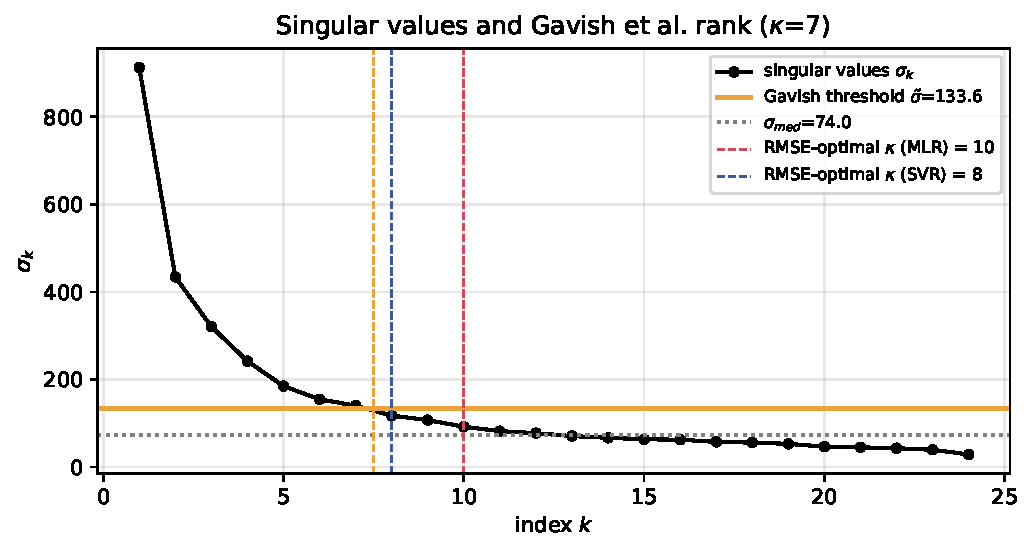
\includegraphics[width=0.7\linewidth]{1_3_gavish.pdf}
\caption{Singular values, Gavish et al.\ threshold and selected ranks.}\label{fig:gavish}
\end{figure}

\begin{table}[h]
\centering
\caption{Denoising results (leave-one-day-out, 104 days).}\label{tab:denoise}
\begin{tabular}{llcccc}
\toprule
Sensor & Method & $\kappa$ & RMSE (\ugm) & $R^2$ & RMSE gain\\
\midrule
MLR & calibrated & -- & 13.42 & 0.876 & --\\
    & TPB-D, RMSE-optimal & 10 & 13.14 & 0.882 & 2.2\%\\
    & TPB-D, Gavish et al. & 7 & 13.28 & 0.879 & 1.1\%\\
\midrule
SVR & calibrated & -- & 12.46 & 0.894 & --\\
    & TPB-D, RMSE-optimal & 8 & 11.65 & 0.907 & 6.5\%\\
    & TPB-D, Gavish et al. & 7 & 11.73 & 0.906 & 5.8\%\\
\bottomrule
\end{tabular}
\end{table}

\paragraph{Discussion.} Denoising helps SVR about three times more than MLR. Projection removes errors that cannot be represented as a typical reference day, such as isolated spikes and hour-to-hour jitter (\cref{fig:dex}). It cannot fix errors that \emph{lie inside} the subspace. The main MLR error is a systematic compression of the amplitude: low days are too high and high days too low. A day with a scaled peak is still a plausible day shape, so the projection leaves it largely untouched. This error would need the linear-mapping (recalibration) step of TPB-C. \Cref{fig:perday} shows that denoising improves 73\% (MLR) and 75\% (SVR) of the days. The largest gains are on the noisiest days, where the calibrated signal has isolated spikes; on days where the calibration is already good the projection changes little. \todo{comment on the days that get worse.}

\begin{figure}[t]\centering
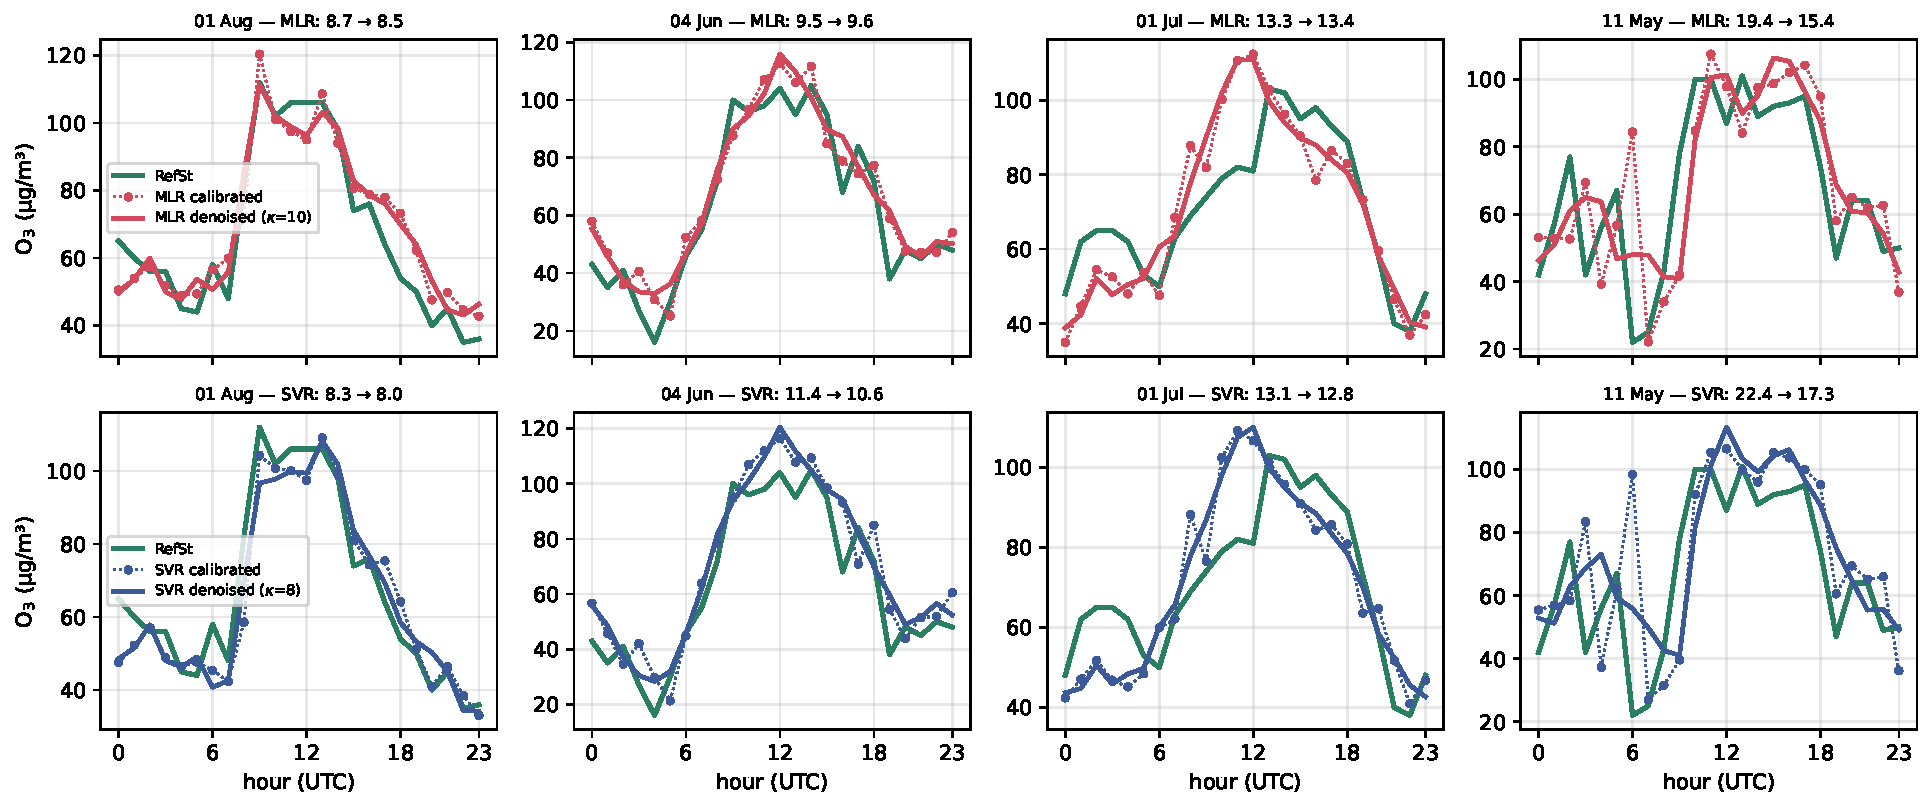
\includegraphics[width=\linewidth]{1_3_examples.pdf}
\caption{Example days before (dotted) and after (solid) denoising with the RMSE-optimal rank. The titles give the daily RMSE before $\to$ after.}\label{fig:dex}
\end{figure}
\begin{figure}[t]\centering
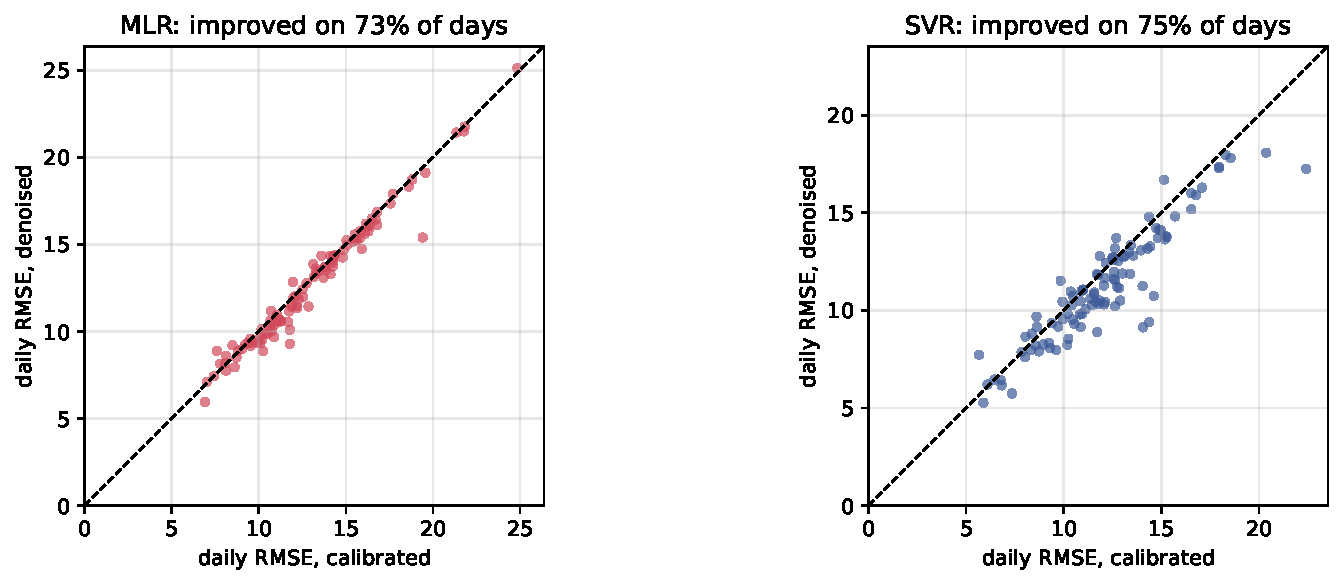
\includegraphics[width=0.85\linewidth]{1_3_per_day.pdf}
\caption{Daily RMSE before vs after denoising. Points below the diagonal are improved days.}\label{fig:perday}
\end{figure}

\subsection{Graph learning}
\Cref{fig:overview} shows the correlations between nodes and their locations. Correlations are high inside the Barcelona cluster, but they also link Barcelona nodes with the Osona nodes, which are 40--78~km away.

\begin{figure}[t]\centering
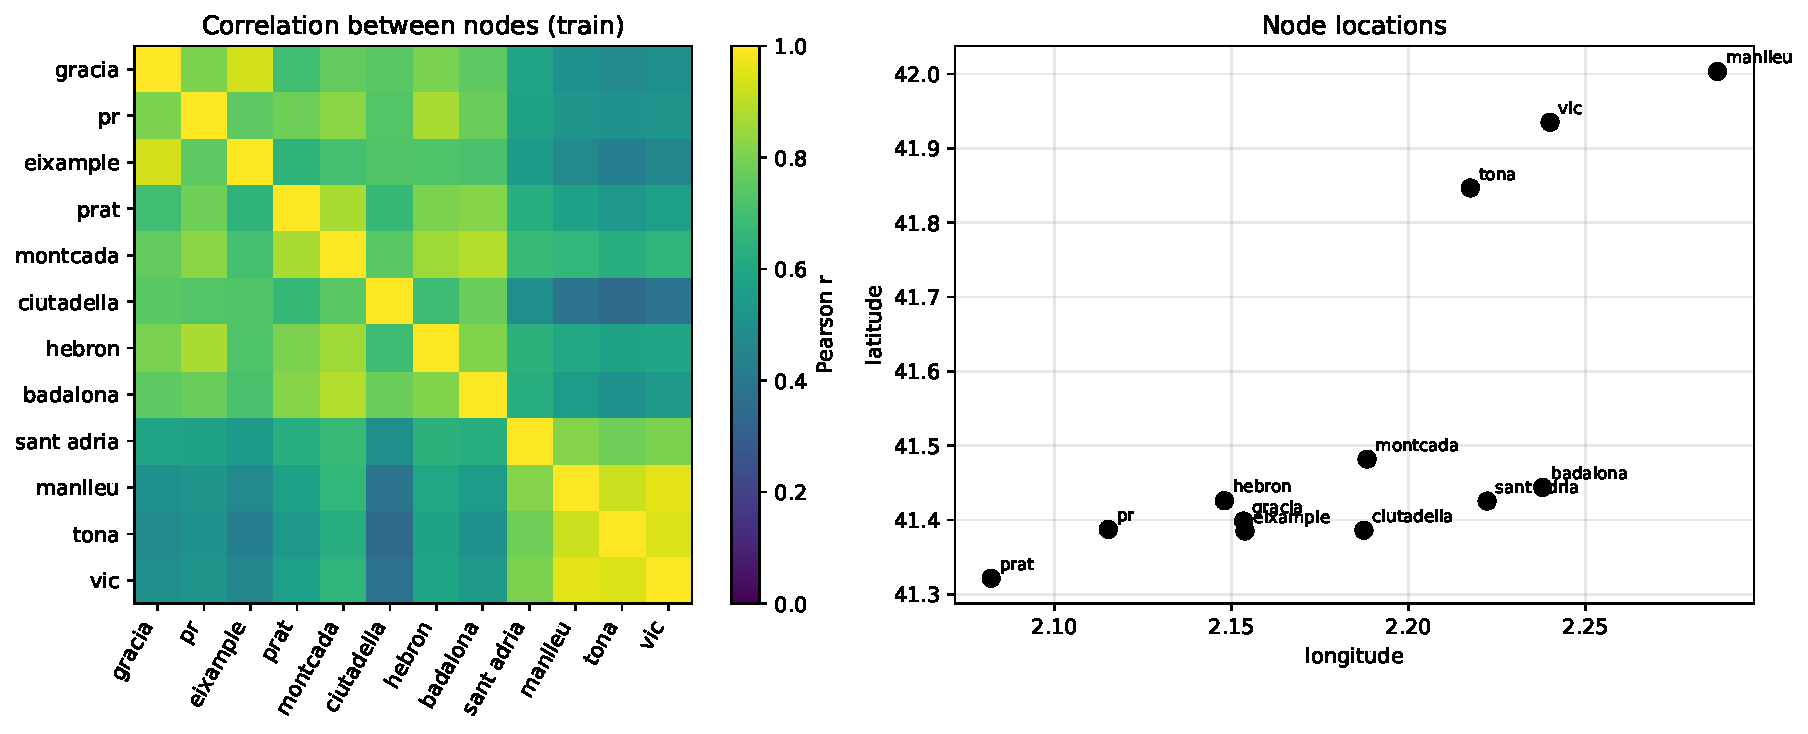
\includegraphics[width=\linewidth]{1_4_overview.pdf}
\caption{Pearson correlation between nodes (training period) and the node locations.}\label{fig:overview}
\end{figure}

\paragraph{Distance-based.} The distance matrix has two clusters (\cref{fig:dist}). Links between the clusters appear only for $T\gtrsim40$~km, and the graph is complete for $T\ge78$~km. Prat is the most isolated node in Barcelona, and Tona is isolated until $T\approx10$~km. With a distance threshold the number of links depends only on $T$. With a weight threshold, a larger $\theta$ shifts the curve towards denser graphs.

\begin{figure}[t]\centering
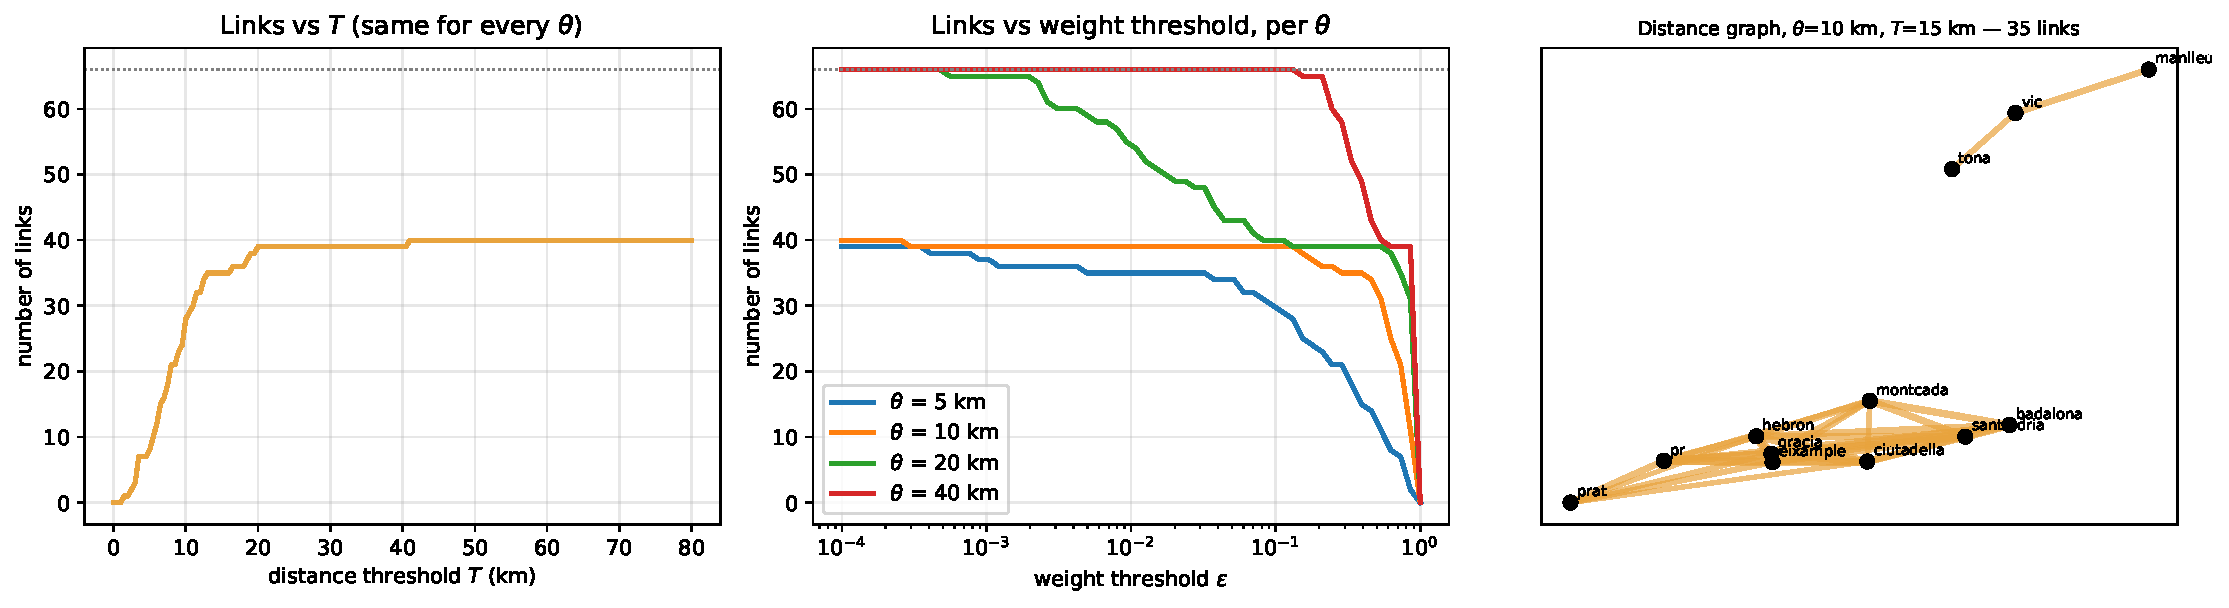
\includegraphics[width=\linewidth]{1_4_distance.pdf}
\caption{Distance-based graph: number of links vs the distance threshold $T$ (left), vs a weight threshold for several $\theta$ (centre), and an example graph (right).}\label{fig:dist}
\end{figure}

\paragraph{GLASSO.} Overall, the number of links decreases with $\lambda$ (\cref{fig:glasso}): about 60 links for $\lambda=10^{-3}$, and an empty graph at $\lambda=1$. On standardised data, every off-diagonal entry is zeroed once $\lambda$ exceeds the largest absolute correlation. The decrease is not monotonic, however. There is a plateau of about 36--40 links for $\lambda\in[0.02,0.1]$, a bump to about 47 links around $\lambda\approx0.3$, and then a steep drop between 0.5 and 1. The precision threshold $T$ shifts the curve by only a few links. \todo{check whether the bump is a convergence artefact (tolerance, \texttt{mode='lars'}) or real.}

\begin{figure}[t]\centering
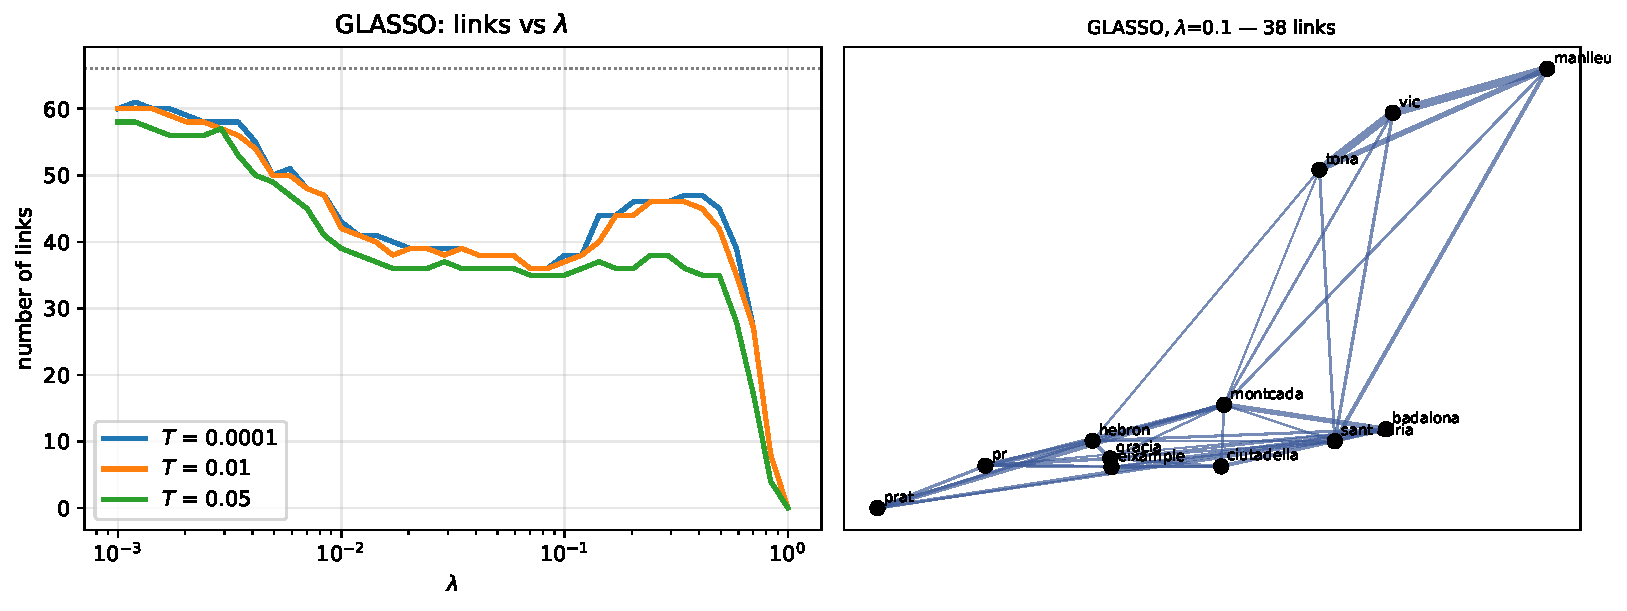
\includegraphics[width=\linewidth]{1_4_glasso.pdf}
\caption{GLASSO: number of links vs $\lambda$ for three precision thresholds (left) and the graph for $\lambda=0.1$ (right).}\label{fig:glasso}
\end{figure}

\paragraph{Laplacian learning.} The number of links grows with $\beta/\alpha$ (\cref{fig:lap}). A small $\beta$ (or large $\alpha$) makes the smoothness term dominate and produces a sparse graph. A large $\beta$ spreads the weight uniformly over many edges, and the graph is complete for $\beta/\alpha\gtrsim1$. For $\alpha=0.1$ and $\alpha=1$ the curves almost coincide, as the first-step analysis predicts. For $\alpha=10$ the alternating $\mathbf Y$-step smooths the data noticeably and changes the curve.

\begin{figure}[t]\centering
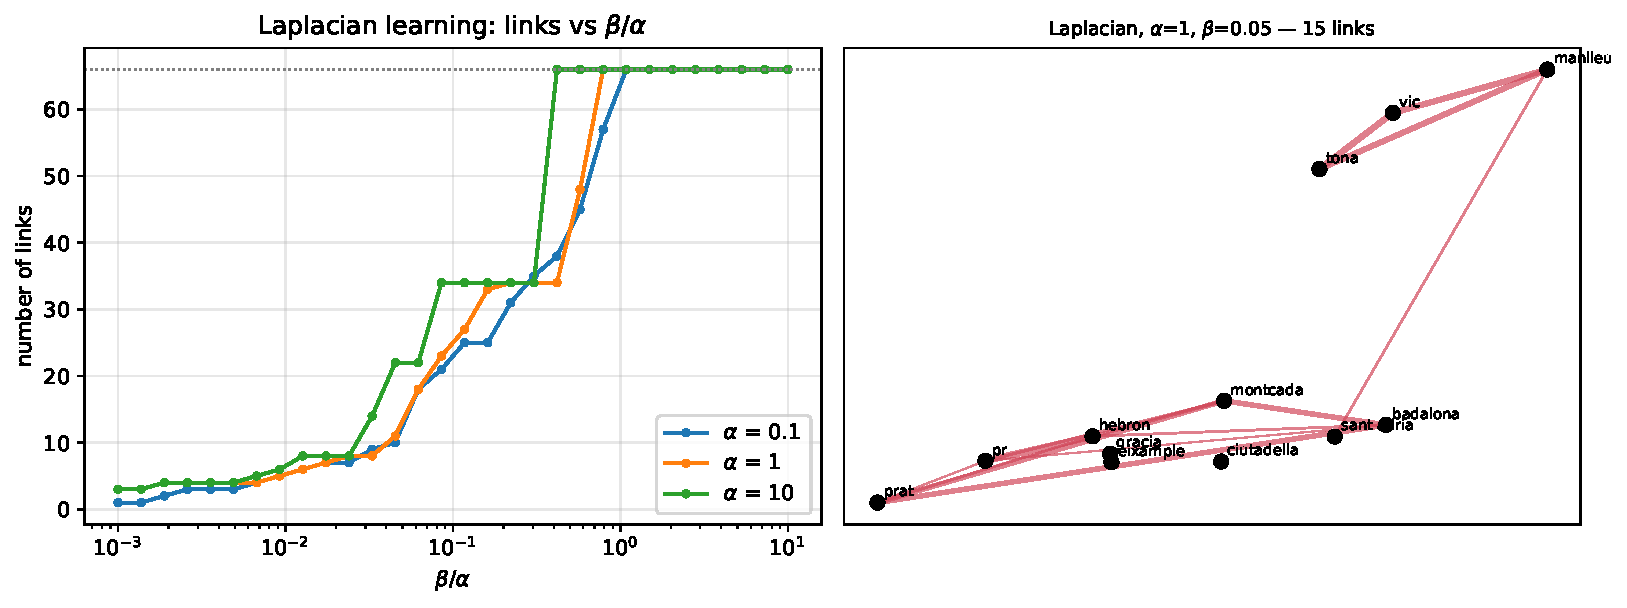
\includegraphics[width=\linewidth]{1_4_laplacian.pdf}
\caption{Laplacian learning: number of links vs $\beta/\alpha$ for several $\alpha$ (left) and an example graph (right).}\label{fig:lap}
\end{figure}

\paragraph{Comparison at equal sparsity.} To compare the methods fairly, each one was tuned to give about 12 (sparse), 24 (medium) and 40 (dense) links (\cref{fig:grid}). At medium density both data-driven graphs connect the two clusters, mainly through Sant Adri\`a. GLASSO keeps a link to Manlleu even in its sparse configuration, whereas the sparse Laplacian graph has no link between the clusters. These long links mean that some distant sites have more similar \Othree{} dynamics than neighbouring urban sites. \todo{interpretation: background vs traffic sites / NO titration.} The distance graph cannot create such links.

\begin{figure}[p]\centering
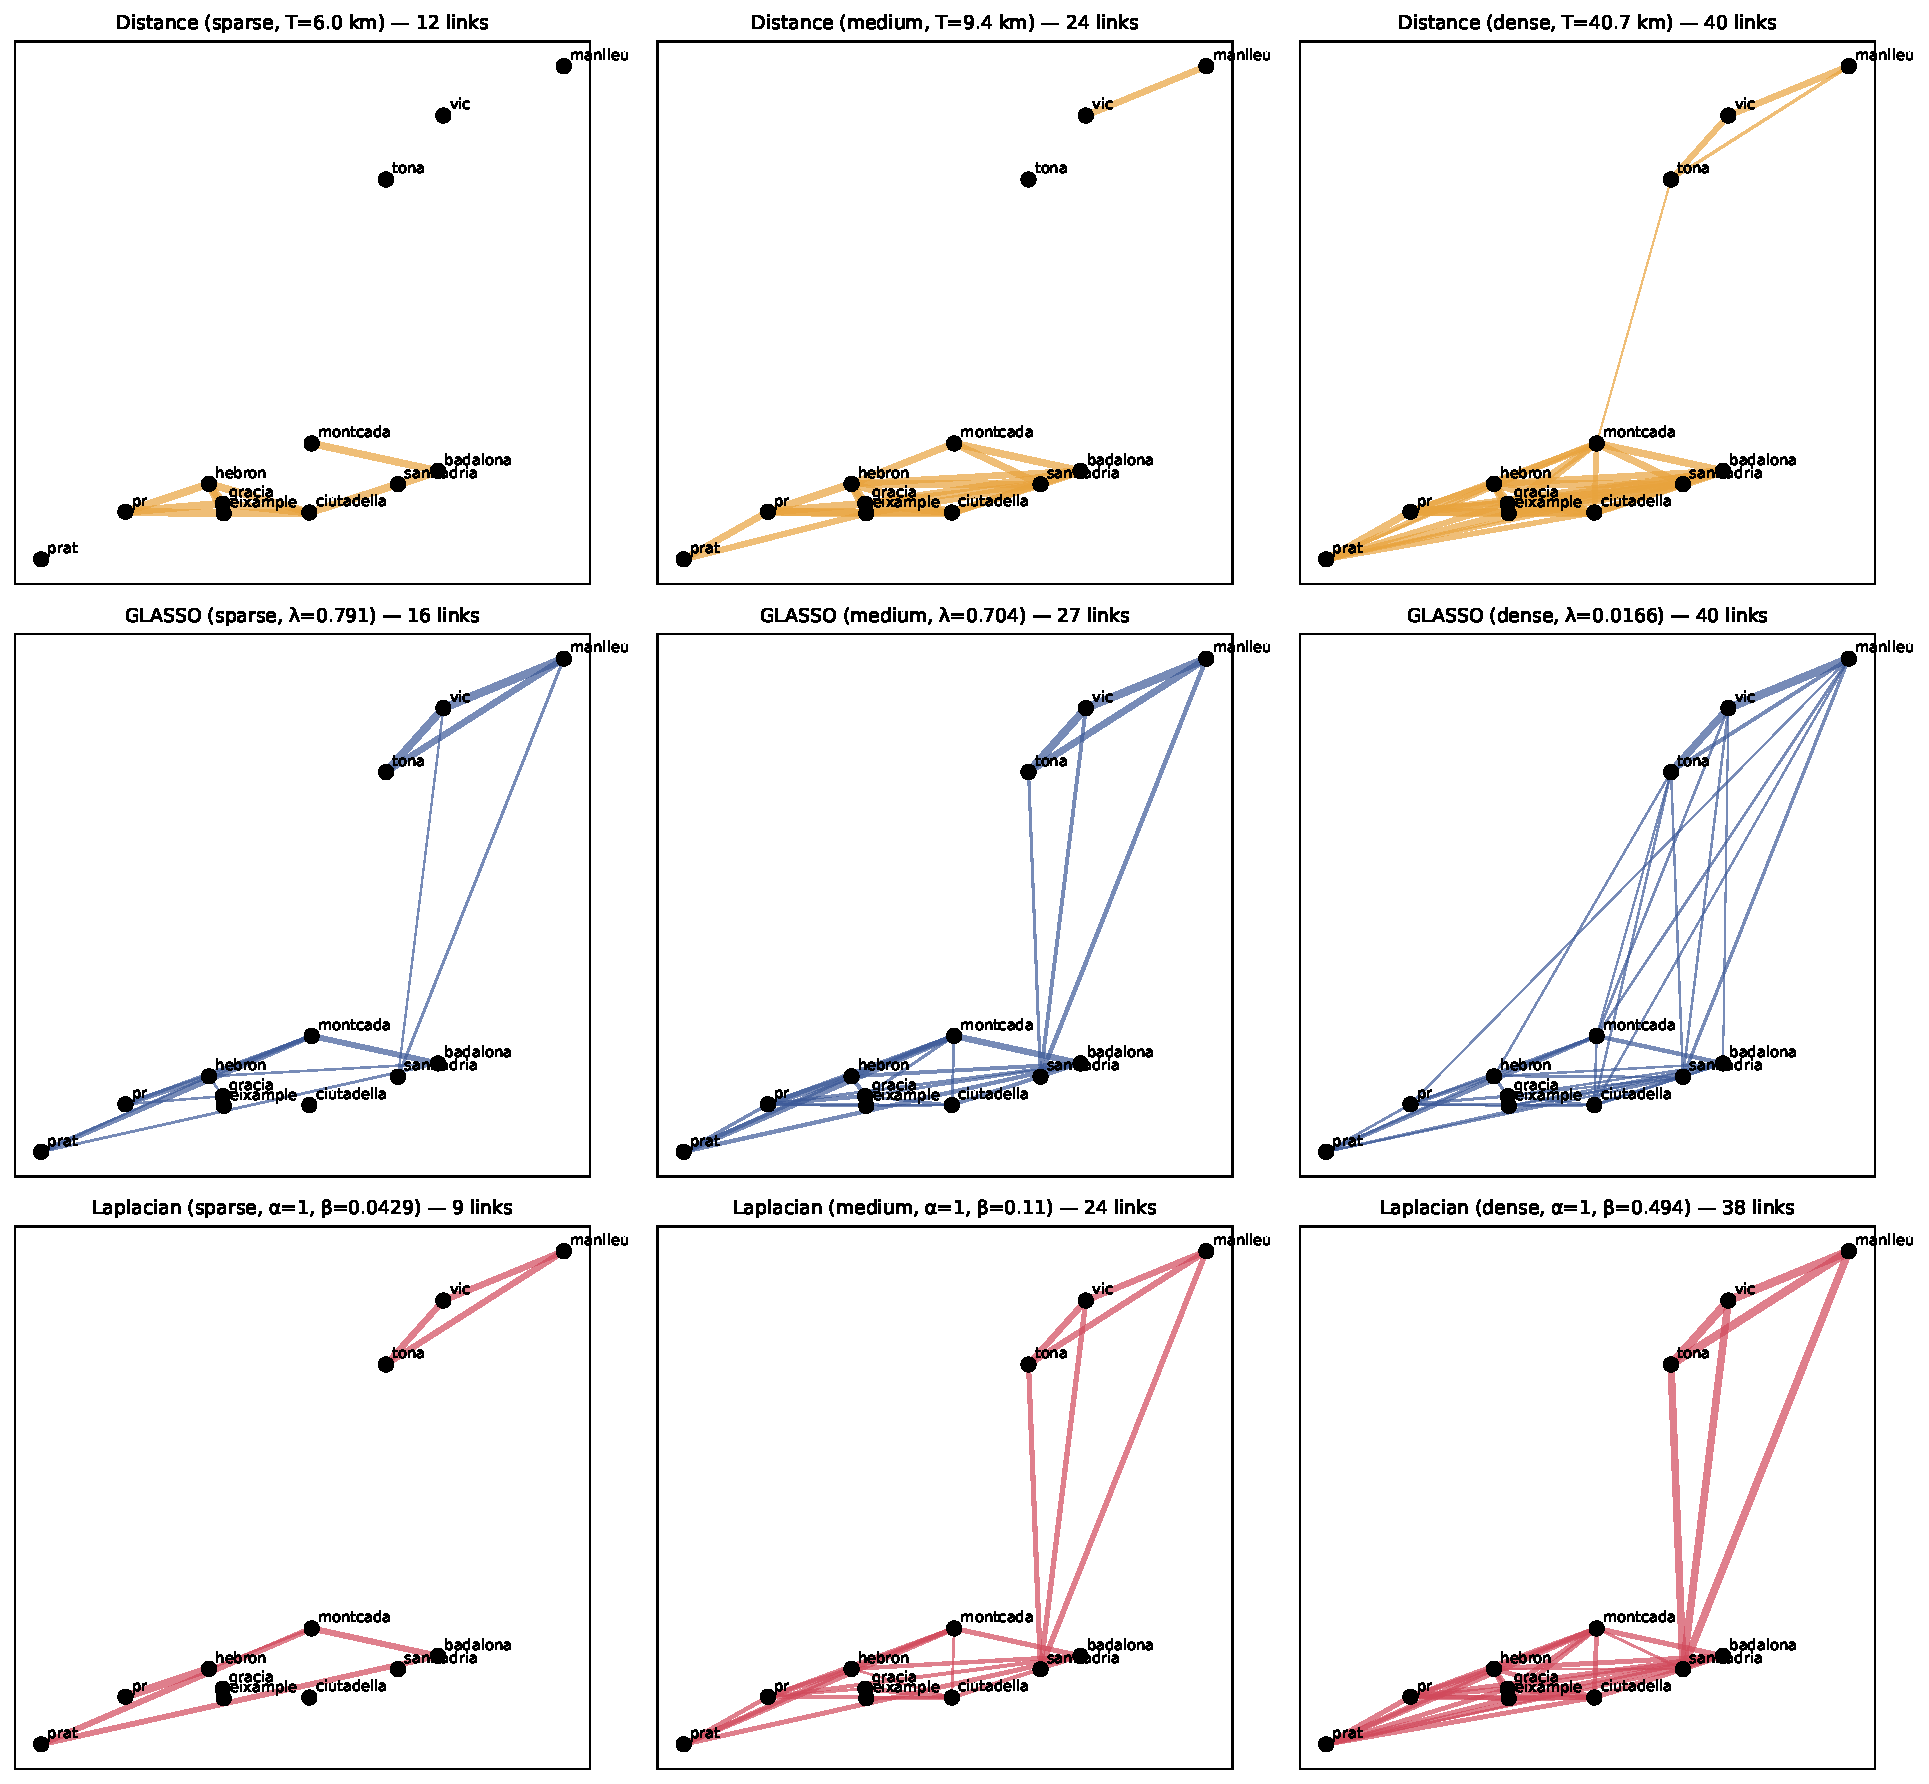
\includegraphics[width=\linewidth]{1_4_graphs_grid.pdf}
\caption{Learned graphs for the three methods (rows) at three sparsity levels (columns). Line width is proportional to the edge weight.}\label{fig:grid}
\end{figure}

\subsection{Virtual sensors}
\Cref{tab:vs} and \cref{fig:vs} summarise the test performance averaged over the 12 target nodes.

\begin{table}[h]
\centering
\caption{Virtual-sensor test performance, averaged over the 12 targets. ``Isolated'' is the number of targets with no neighbours, which are predicted with the training mean.}\label{tab:vs}
\begin{tabular}{llccccc}
\toprule
Graph & Level & Mean deg. & Isolated & RMSE MLR & RMSE SVR & $R^2$ SVR\\
\midrule
Distance  & sparse & 2.0 & 4 & 21.53 & 21.35 & 0.382\\
          & medium & 4.0 & 1 & 15.23 & 15.12 & 0.662\\
          & dense  & 6.7 & 0 & 12.17 & 12.26 & 0.781\\
GLASSO    & sparse & 2.7 & 1 & 12.87 & 12.68 & 0.740\\
          & medium & 4.5 & 0 & 11.82 & \textbf{11.62} & \textbf{0.805}\\
          & dense  & 6.7 & 0 & \textbf{11.61} & 11.82 & 0.800\\
Laplacian & sparse & 1.5 & 2 & 14.43 & 14.40 & 0.657\\
          & medium & 4.0 & 0 & 11.85 & 11.66 & 0.804\\
          & dense  & 6.3 & 0 & 11.67 & 11.76 & 0.801\\
\midrule
Full mesh & --     & 11  & 0 & 11.69 & 12.11 & 0.793\\
Full mesh, Ridge / Lasso & -- & 11 & 0 & 11.67 / 11.60 & -- & --\\
\bottomrule
\end{tabular}
\end{table}

\begin{figure}[t]\centering
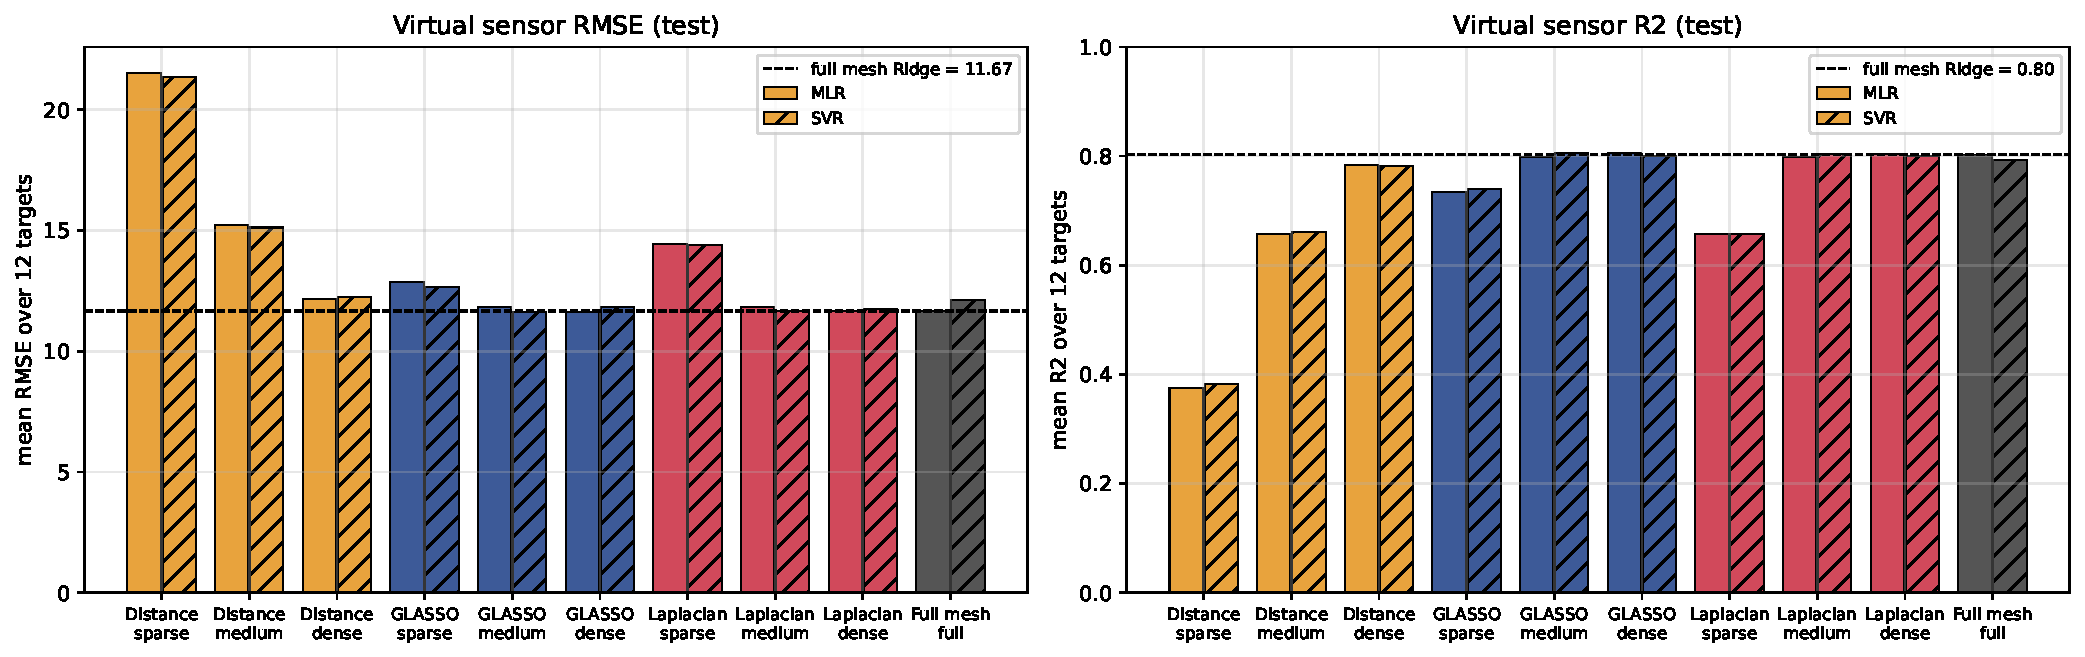
\includegraphics[width=\linewidth]{1_4_vs_summary.pdf}
\caption{Mean virtual-sensor RMSE and $R^2$ over the 12 targets for each graph and sparsity level. The dashed line is the full-mesh Ridge baseline.}\label{fig:vs}
\end{figure}
\begin{figure}[t]\centering
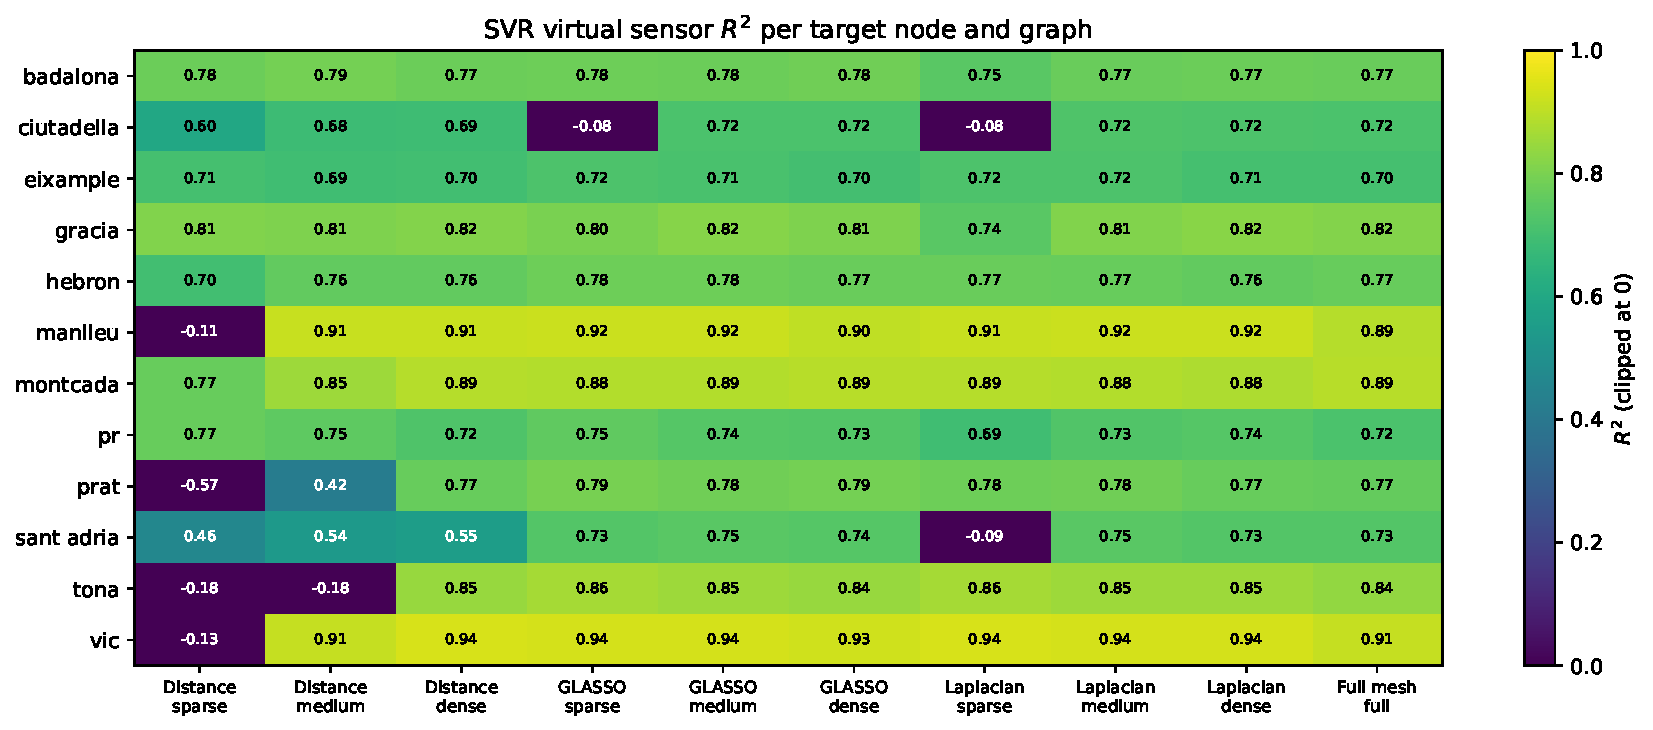
\includegraphics[width=\linewidth]{1_4_vs_heatmap.pdf}
\caption{SVR virtual-sensor $R^2$ per target node and graph.}\label{fig:vsheat}
\end{figure}

The main findings are:
\begin{itemize}
  \item \textbf{Data-driven neighbourhoods are much more efficient.} With about 4 neighbours, the GLASSO and Laplacian graphs already match the full mesh ($R^2\approx0.80$). The distance graph needs about 7 neighbours to come close.
  \item \textbf{Sparse distance graphs fail} mainly because of isolated nodes. Prat, Tona, Vic and Manlleu have no neighbour within 6~km. Where neighbours do exist, the median $R^2$ is less affected than the mean (\cref{fig:vsheat}).
  \item \textbf{Regularisation of the full mesh brings little} (11.69 vs 11.60--11.67), because 11 features and 1\,519 samples are far from overfitting. However, the graph gives an interpretable sparse model that needs fewer sensors to be available.
  \item \textbf{MLR and SVR perform similarly}, which suggests that the spatial relation between \Othree{} sites is close to linear. \todo{check per-node differences; consider GP.}
\end{itemize}

\begin{figure}[t]\centering
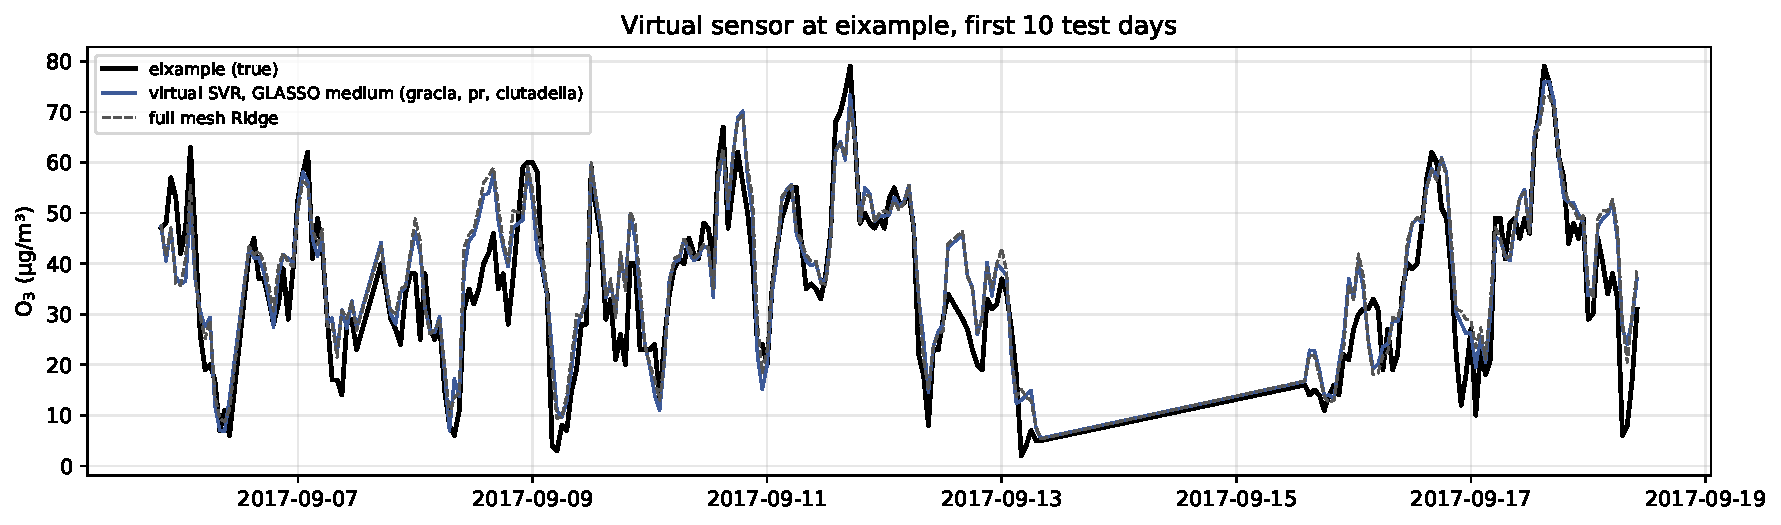
\includegraphics[width=\linewidth]{1_4_vs_example.pdf}
\caption{Virtual sensor at Eixample: SVR with the GLASSO-medium neighbourhood vs the full-mesh Ridge model, over the first 10 test days.}\label{fig:vsex}
\end{figure}

%=====================================================================
\section{Conclusions}\label{sec:conclusions}
%=====================================================================
\begin{itemize}
  \item The daily \Othree{} profiles of a reference station lie close to a low-dimensional subspace: 7--10 of the 24 dimensions suffice. Projecting calibrated LCS days onto this subspace reduces the RMSE of an SVR-calibrated sensor by 6.5\% and that of an MLR-calibrated sensor by 2.2\%.
  \item Denoising removes errors that are inconsistent with plausible day shapes, but not systematic amplitude errors. This explains why it helps MLR less, and it motivates the additional linear-mapping step of TPB-C.
  \item The Gavish--Donoho threshold gives $\kappa=7$ without any co-located ground truth. It is stable across folds and only about 0.1~\ugm{} worse than the RMSE-optimal rank, so it is a practical choice for deployments without a reference instrument nearby.
  \item For virtual sensors, graphs learned from the data (GLASSO, Laplacian) produce better neighbourhoods than geographic distance. With about 4 neighbours per node they match the full-mesh model, while sparse distance graphs leave nodes isolated.
  \item \todo{limitations: single campaign/season; rank chosen on the evaluation days; future work: TPB-C, GP virtual sensors, robustness to missing neighbours.}
\end{itemize}

%=====================================================================
\begin{thebibliography}{99}\small
\bibitem{ferrercid2021} P.~Ferrer-Cid, J.~M. Barcel\'o-Ordinas, J.~Garc\'ia-Vidal, ``Graph learning techniques using structured data for IoT air pollution monitoring platforms,'' \emph{IEEE Internet of Things Journal}, vol.~8, no.~17, pp.~13652--13663, 2021.
\bibitem{friedman2008} J.~Friedman, T.~Hastie, R.~Tibshirani, ``Sparse inverse covariance estimation with the graphical lasso,'' \emph{Biostatistics}, vol.~9, no.~3, pp.~432--441, 2008.
\bibitem{dong2015} X.~Dong, D.~Thanou, P.~Frossard, P.~Vandergheynst, ``Laplacian matrix learning for smooth graph signal representation,'' in \emph{Proc. IEEE ICASSP}, 2015, pp.~3736--3740.
\bibitem{dong2016} X.~Dong, D.~Thanou, P.~Frossard, P.~Vandergheynst, ``Learning Laplacian matrix in smooth graph signal representations,'' \emph{IEEE Trans. Signal Processing}, vol.~64, no.~23, pp.~6160--6173, 2016.
\bibitem{kalofolias2016} V.~Kalofolias, ``How to learn a graph from smooth signals,'' in \emph{Proc. AISTATS}, 2016.
\bibitem{shuman2013} D.~I. Shuman, S.~K. Narang, P.~Frossard, A.~Ortega, P.~Vandergheynst, ``The emerging field of signal processing on graphs,'' \emph{IEEE Signal Processing Magazine}, vol.~30, no.~3, pp.~83--98, 2013.
\bibitem{stankovic2019} L.~Stankovi\'c et al., ``Understanding the basis of graph signal processing via an intuitive example-driven approach,'' arXiv, 2019.
\bibitem{turk1991} M.~Turk, A.~Pentland, ``Eigenfaces for recognition,'' \emph{Journal of Cognitive Neuroscience}, vol.~3, no.~1, pp.~71--86, 1991.
\bibitem{gavish2014} M.~Gavish, D.~L. Donoho, ``The optimal hard threshold for singular values is $4/\sqrt3$,'' \emph{IEEE Trans. Information Theory}, vol.~60, no.~8, pp.~5040--5053, 2014.
\bibitem{spinelle2015} L.~Spinelle, M.~Gerboles, M.~G. Villani, M.~Aleixandre, F.~Bonavitacola, ``Field calibration of a cluster of low-cost available sensors for air quality monitoring. Part A: Ozone and nitrogen dioxide,'' \emph{Sensors and Actuators B}, vol.~215, pp.~249--257, 2015.
\bibitem{castell2017} N.~Castell et al., ``Can commercial low-cost sensor platforms contribute to air quality monitoring and exposure estimates?'' \emph{Environment International}, vol.~99, pp.~293--302, 2017.
\end{thebibliography}

\end{document}
